%\documentclass[12pt,a4paper]{report}
%\usepackage{graphicx}
%
%\setcounter{tocdepth}{4}
%\setcounter{secnumdepth}{4}
%\usepackage{subfig}
%\usepackage{listings}
%\graphicspath{ {/home/ram/Documents/20170423/figures/} }
%\begin{document}
\chapter{Porting of image processing and computer vision algorithms}
The image processing and computer vision algorithms are useful in defence, entertainment, digital security, etc. The data being processed in these fields is huge. So,  High-performance implementations of these algorithms are needed to run them quickly and accurately in real time. One of the applications this work is aimed at is to process the data from UAV(Unmanned Aerial Vehicle). The data from the UAV will be sent for processing to Automated Ground Control System(AGCS).  
\section{Components in the AGCS}
The Figure \ref{Hies target hardware} shows the list of different hardware components connected together to form a High-performance computing platform. The Single Board Computer (SBC) acts as a master and other hardware works in conjunction with SBC as slaves. From the Figure we can see a GPGPU hardware block on which this work is aimed at. AGCS follows a typical client-server architecture. The clients are with less processing power than the server. In this work GPGPU is the target hardware component to exploit the performance.
\begin{figure}[h!]
	\centering
	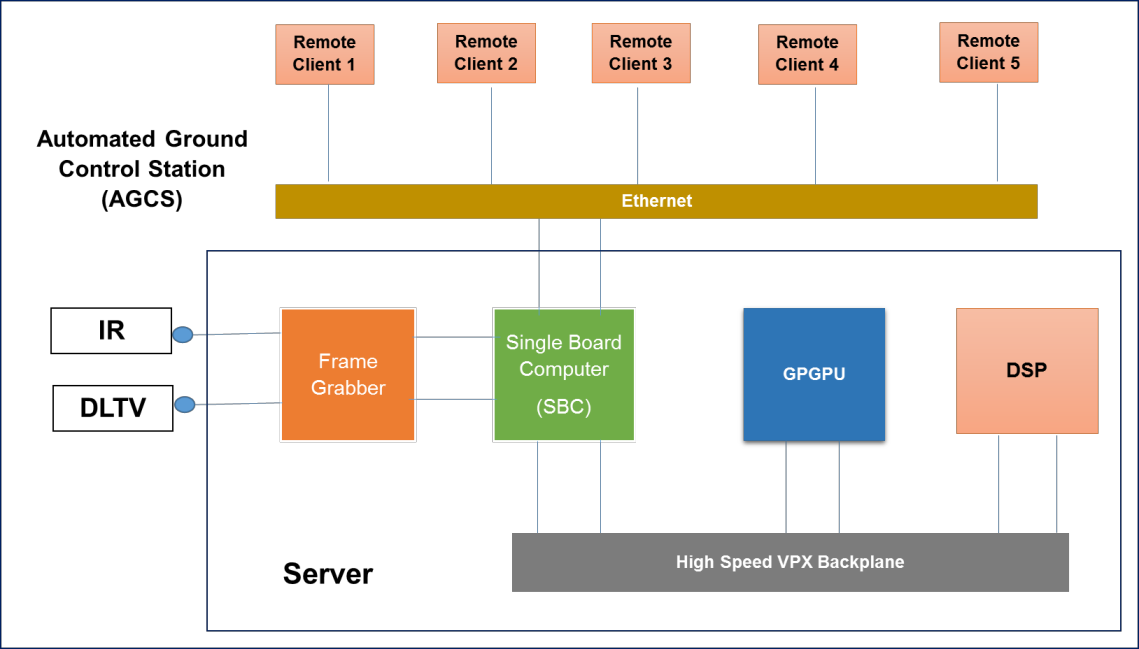
\includegraphics [width=\linewidth]{TargetHardwareHIES.png}
	\caption{The different hardware components in automated ground control system}
	\label{Hies target hardware}
\end{figure}
\section{Adaptive contrast Enhancement}
Contrast enhancement is used to increase the contrast of an image for better visual appearance. Histogram equalization can perform contrast enhancement, but it also enhances the noise in the image.  So adaptive contrast enhancement algorithm is developed to avoid the noise component amplification.
\subsection{Algorithm Flow}
In the following, the algorithm flow of Adaptive contrast Enhancement is explained with references. In this work, high performance implementation of this algorithm is designed to get best performance using GPGPU computing. 
\begin{itemize}
	\item The first stage in this algorithm is, converting the input image with RGB model to HSV colour model. It is easy to work with only the luminance component V. The components H, S and V can be computed using the Equations \ref{Seq},\ref{Veq} and \ref{Heq}. In the case of YUV color model images, only Y component is sufficient to process.
	\begin{equation}\label{Seq}
	S=
	\begin{cases}
	0, & \text{if}\ max=0 \\
	\frac{max-min}{min} \times 255, & \text{otherwise}
	\end{cases}
	\end{equation}
	\begin{equation}\label{Veq}
	V = max \times 255	
	\end{equation}
	\begin{equation}\label{Heq}
		H=
		\begin{cases}
		\text{undefined}, & \text{if}\ max=min \\
		60^o \times \frac{g-b}{max-min}+0^o, & \text{if} max= r \&\& g\geq b \\
		60^o \times \frac{g-b}{max-min}+360^o, & \text{if} max= r \&\& g < b \\
		60^o \times \frac{b-r}{max-min}+120^o, & \text{if} max= g \\
		60^o \times \frac{r-g}{max-min}+240^o, & \text{if} max= b \\
		\end{cases}
	\end{equation}
		
		\item Then for the luminance component V histogram $H_v(x_k)$ is calculated. where $x_k$ represents the \textit{kth} brightness level and $n_k$ is the pixels count in the image having brightness level $x_k$.
		\begin{equation}\label{histeq}
		H_v(x_k)=n_k
		\end{equation}
		\item The luminance histogram is smoothed with a gaussian kernel. This is a gaussian convolution and depends on the pixel intensity(x) and standard deviation ($\sigma_g$). The standard deviation calculation is explianed in \cite{ACE}. The Equation \ref{gausseq} gives operation of gaussian convolution.
			\begin{equation}\label{gausseq}
			\begin{split}		
			S_{HV}(x,\sigma_g)&=H_v(x)*g(x,\sigma_g)=\int_{-\infty}^{\infty} 	H_v(u)g(x-u,\sigma_g)du\\
			&=\int_{-\infty}^{\infty} 	H_v(u) \frac{1}{\sqrt{2\pi\sigma_g}} \exp^\frac{(x-u)^2}{2{\sigma_g}^2}
			\end{split}
			\end{equation}
			\item The average differences are employed on the smoothed histogram to find the major peaks and valleys. The positive to negative crossover gives a peak while the negative to positive crossover gives a valley. The Equation \ref{smootheq} shows the avergae difference operation.
			\begin{equation}\label{smootheq}
			S_{HV}(x)=\frac{1}{\sigma_g - 1}\sum_{i=1}^{\sigma_g - 1}\frac{S_{HV}(x+i)-S_{HV}(x-i)}{2\times i}
			\end{equation}
			
		\item Piece-wise linear transformation for k-1 line segments is given by Equation \ref{PLTeq}. The number of line segments are decided by the number of luminance distributions. Let there are k luminance distributions \{$p_1,p_2,....,p_k$\}, then the line segments are $k+1$.
		\begin{equation}\label{PLTeq}
		T_{k-1} =\frac{(y_k-y_{k-1})}{x_k-x_{k-1}} \times {(x-x_{k-1})} +y_{k-1}
		\end{equation}
		The $k$ luminance distributions need $2k$ parameters to set. But in APFPLT the input parameters are the valleys \{$v_0,v_1,v_2,...,v_k$\}, and the output parameters are calculated using the Equation \ref{probeq}. The $Pr(x)$ is the probability of the luminance distribution.
		\begin{equation}\label{probeq}
		y_k = \sum_{S}^{v_k} Pr(x) \times 255	
		\end{equation}  

\end{itemize}
\begin{figure}[htb]
	\centering
	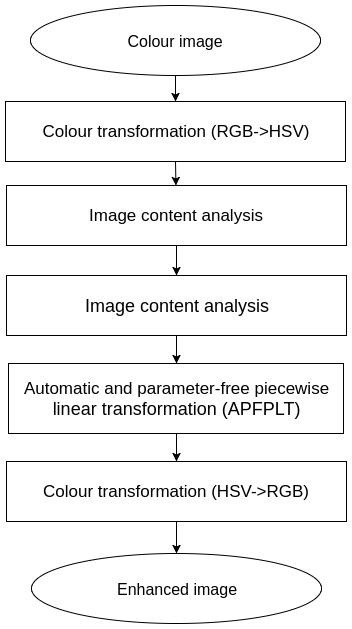
\includegraphics[width=0.5\linewidth]{ACEblockdiagram.png}
	\caption{Adaptive contrast enhancement algorithm flow}
	\label{ACE}
\end{figure}
\subsection{GPGPU Implementation}
\begin{itemize}	
		\item Histogram calculation is shown in Equation \ref{histeq}, the output size is the number of bins used to hold the pixel frequencies. A bin represents a single intensity level or a group of intensities. So the range of bin size varies from 1 to 255.
		\item So all the pixels in an image contributes to maximum 255 bins. In this case the increment operation has to take place. So it breaks the parallelism.
		\item A block of 32x32 threads is selected. For an image of size 640x480,  a grid of 20x15 blocks is created to complete the histogram calculation.
		\item The histogram is smoothened using a gaussian mask calculated using Equation \ref{gausseq}. 
		Since this operation is element wise then the dataparallelism can be extraced here. if each thread contributes a single output then, output size work threads will complete the operation on all entire elements in parallel.
		 \item After having the required information, the PLT is implemented on GPU with full parallelism. From the equation \ref{PLTeq}, the PLT operation is independent of other outputs. The output size number of threads can concurrently work to compute all the outputs.
\end{itemize}
\subsection{Results and Discussions}
The above implementation is tested against different image data and good speedups are observed. The Table \ref{timing of ace} gives the timing performance of the algorithm. The speed up found in Table \ref{timing of ace} is the ratio of CPU timing to the CPU-GPU timing. From Table \ref{timing of ace} we can observe that the speed up has a positive linear relationship with input size. 
\begin{figure}[htb]
\centering
\subfloat[input]{{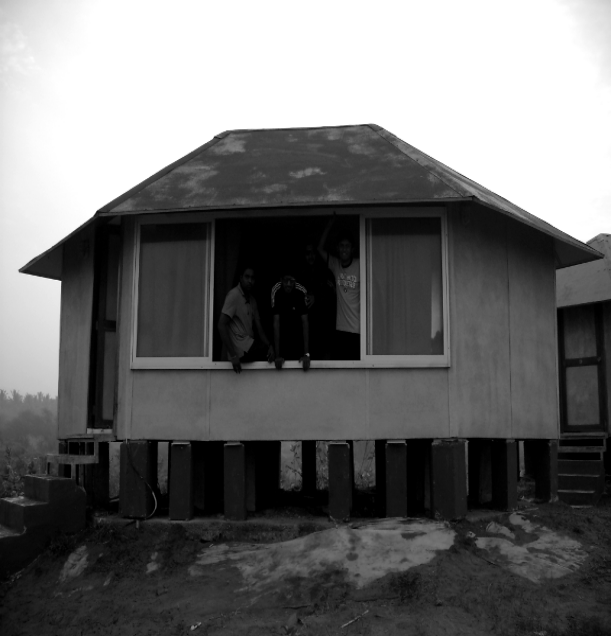
\includegraphics[width=6cm]{aceinput.png} }}%
\qquad
\subfloat[output]{{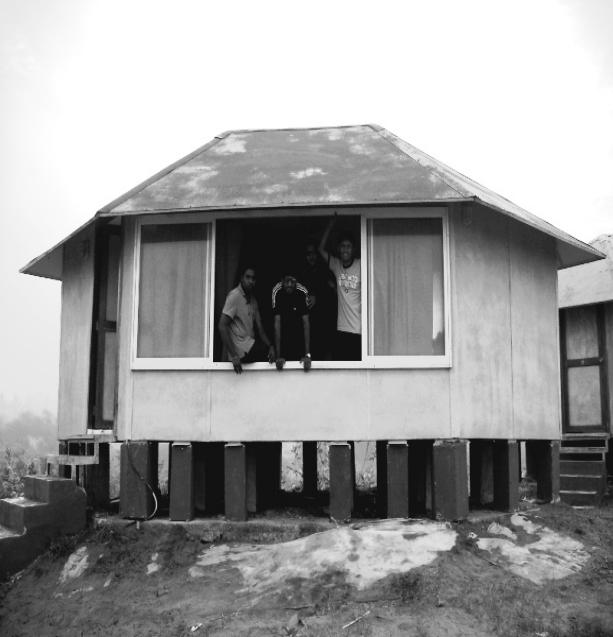
\includegraphics[width=6cm]{aceoutput.png} }}%
\caption{Adaptive contrast enhancement functional results}%
\label{fig:ace results}%
\end{figure}
\begin{table}[htb]
\centering
\begin{tabular}{ |c|c|c|c| }
\hline
\textbf{Image Resolution} & \textbf{CPU(in ms)} &  \textbf{GPU(in ms)} & \textbf{Speed Up}\\
\hline
640 X 48 & 18.73 & 3.23 & 6x \\
\hline
1280 x 72 & 55.27 & 6.17 & 9x \\
\hline
1920 x 1080 & 104.54 & 11.74 & 9x \\
\hline
\end{tabular}
\caption{Timing performance of Adaptive contrast enhancement algorithm.}
\label{timing of ace}
\end{table}
\section{Motion De-blur algorithm}
Restoration of blurred images is useful in consumer-level photography, medical imaging and astronomy. One of the reasons for the Blur in an image is due to the motion of the camera and is called the motion blur. Motion blur in images happens when there exist a relative motion between the camera and an object. 
\subsection{Motion blur}
Blur distorts the details in the image. The original image can be restored from the blurred image, if we have the blur kernel. The blur kernel estimation depends on the blur motion and direction in the blurred image. Deconvolving blurred image with the blur kernel gives the original image. This process of Image restoration is called de-blurring. The deblurring methods are categorised based on the deconvolution used. The deconvolution methods available for deblurring are non-iterative Weiner algorithm \cite{Blurred image restoration} and iterative Lucy-Richardson, sparse method, etc. In this work sparse deconvolution is used.
\subsection{Algorithm Flow}
In the following, the algorithm flow of Motion De-blur is explained with references. In this work, high performance implementation of this algorithm is designed to get best performance using GPGPU computing. 
\begin{enumerate}
	\item Blur kernel estimation
	\item Deconvolution 
\end{enumerate}
\subsubsection{Blur kernel estimation}
In finding blur kernel there are two stages, calculating blur angle and calculating blur length. In calculating the blur angle following are the different stages.

	%\item{\textbf{Gradient of the Image}} \hfill \break
	\paragraph*{Gradient of the Image} \hfill \newline	
	Gradient is the directional change of a scalar; here the gradient is used to find the directional change in the image intensities. The gradient of the image is simply the edge detection. Generally the edges contain useful data about blur parameters, so processing only on the edges is more easy than the entire image \cite{Blurred image restoration}.
	\vspace{0.2cm} \par{}From the equation \ref{gradeq} the image gradient $(G)$ is the magnitude of horizontal$(G_x)$ and vertical gradient$(G_y)$. For an image of size $N\times M$, $f(x,y)$ represents the image intensity at location $(x,y)$, where $x$ varies from $1,.....,N$ and $y$ varies from $1,....,M$.
	\begin{equation}
	G_x=\frac{f(x+1,y) - f(x-1,y)}{2}
	\end{equation}
	\begin{equation}
	G_y=\frac{f(x,y+1) - f(x,y-1)}{2}
	\end{equation}
	\begin{equation}\label{gradeq}
	G = \sqrt{{G_x}^2+{G_y}^2}
	\end{equation}
	
	%\item{\textbf{Power spectrum calculation}} \hfill \break
	\paragraph*{Power spectrum calculation} \hfill \\
	The power spectrum of the image gradient contains a regular structure which has a relationship with the length and angle of the blur \cite{Blurred image restoration}. With the properly filtered power spectrum, the length and blur can be found accurately. The power spectrum is shifted such that all the zero frequencies are aligned at the centre of the image.
	\paragraph*{} The 2-Dimensional Discrete Fourier Ttransform can be calculated using the Equation \ref{pseq}.
	\begin{equation}\label{pseq}
	F(u,v)=\sum_{x=1}^{N}\sum_{y=1}^{M}f(x,y) \exp^{\omega_N (x-1)(u-1)} \exp^{\omega_M (y-1)(v-1)}
	\end{equation}
	where $\omega_M=-\frac{2\pi i}{M}$, $\omega_M=-\frac{2\pi i}{N}$ and $F(u,v)$ represents the output spectrum.
	\paragraph*{Bandpass Filtering} \hfill \break
	%\item{\textbf{Bandpass Filtering}} \hfill \break
	 The band-pass Butterworth filter can be designed by cascading two Butterworth filters, a Low pass and a High pass. First, a Low pass filtering is done on the input and then a High pass filtering follows. The discrete form of Butterworth low pass filter can be found by using the Equation \ref{bwfeq}. The variable $D(u,v)$ is the operating frequency, $d$ is the cut-off frequency and $n$ is the order of the filter.	
	
	\begin{equation}\label{bwfeq}
	%H(u,v)=1-\frac{1}{{1+[\frac{D(u,v)W}{{D^2}(u,v)-{D_0}^2}]}}
	%G^2\big(w) = \frac{G_0^2}{\big(1+\big(\frac{\omega}{\omega_c}\big)^{2 n}\big)}
	G\big(u,v) = \frac{1}{\big(1+\big(\frac{D(u,v)}{d}\big)^{2 n}\big)}
	\end{equation}
	 \par\noindent \vspace{0.2cm}
	\begin{equation} \label{dist}
	D(u,v)=\sqrt{(u-M/2)^2+(u-N/2)^2}
	\end{equation}
	where $N,M$ are width and height of the image respectively.

	\paragraph*{Radon Transform} \hfill \break
%	\item{\textbf{Radon Transform}} \hfill \break
	The Radon transform operates on the filtered power spectrum. It finds the parallel stripes from the pattern contained in the power spectrum. The Radon transform finds the projections of the data for a given angle as shown in Equation \ref{radoneq}, this continues for several selected angles. The angle at which maximum occcurs in the radon transform output gives the blur angle.
	\begin{equation}\label{radoneq}
	R_\theta(x')=\sum_{-\infty}^{\infty} f(x'\cos\theta-y'\sin\theta,x'sin\theta + y'\cos\theta)
	\end{equation}
	where 
	
	$\begin{bmatrix}
		x'\\
		y'\\
	\end{bmatrix} = \begin{bmatrix}
	cos\theta & sin\theta \\
	-sin\theta & cos\theta
	\end{bmatrix}$ 
	
\begin{figure}[h!]
	\centering
	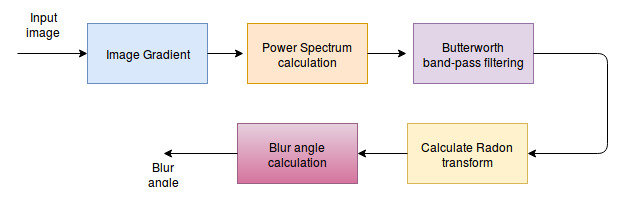
\includegraphics[width=\linewidth]{blur_angle_md.jpg}
	\caption{Block-diagram for calculating blur angle in motion de-blur algorithm}
	\label{blur angle}
\end{figure}
	\paragraph*{Estimate the Target function} \hfill \break
	%\item {\textbf{Estimate the Target function}} \hfill \break
	The spatial domain image is converted into the spectral domain and a log transform is applied, which is then converted back to the spatial domain. The converted data is rotated with the estimated blur angle, a vector is formed by averaging all the columns in the rotated data. This vector is called target function which contains the information regarding the blur length.
	\paragraph*{Blur length calculation} \hfill \break
	%\item {\textbf{Blur length calculation}}
	The target function is as shown in the figure \ref{target function} also illustrates the blur length calculation. The distance d has inverse relationship with the blur length. For an image of MxM size, the blur length can be calculated using the Equation \ref{blurlengtheq}.
	\begin{equation}\label{blurlengtheq}
		Blur length = \frac{M}{d}
	\end{equation}
	\begin{figure}[h!]
		\centering
		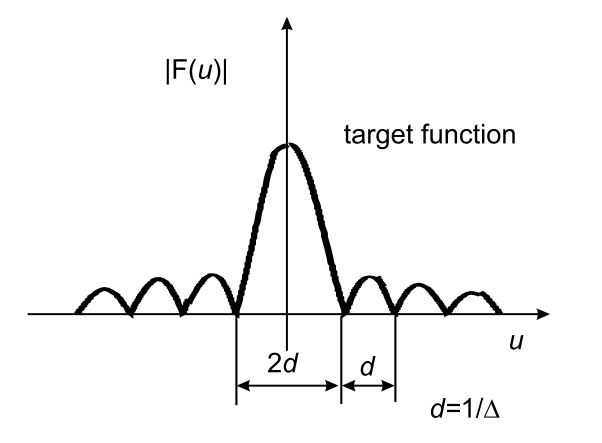
\includegraphics[width=0.5\linewidth]{targetFun.png}
		\caption{Target function for calculating blur length in motion de-blur algorithm}
		\label{target function}
	\end{figure}
	\begin{figure}[h!]
		\centering
		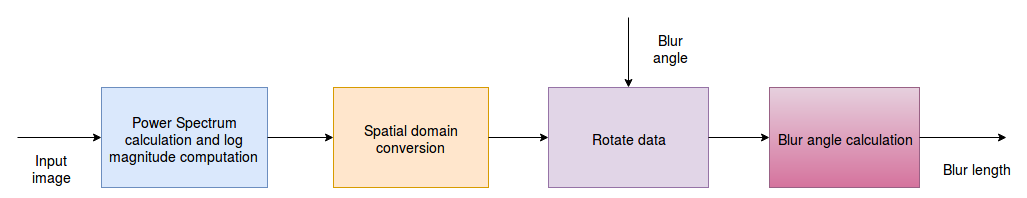
\includegraphics[width=\linewidth]{blur_length_md.png}
		\caption{block-diagram for Calculating blur length in motion de-blur algorithm}
		\label{blur length}
	\end{figure}
	\paragraph*{Blur kernel estimation} \hfill \break
%	\item {\textbf{Blur kernel estimation}}
	With the known blur length and blur blur angle the point spread function(PSF) can be found. Since the generation of PSF takes a very time on CPU so it is not a targeted portion for parallel implementation.
%\end{itemize}
\subsubsection{Deconvolution}
The deconvoluton of blurred image with the estimated blur kernel gives the de-blurred image. The sparse method based deconvolution is used in this algorithm. It contains a series of convolutions with the static kernels and blur kernel. The convolutions will iterate multiple times for estimating the correct input.\par\noindent
Kernel1 = [-1,1] \par\noindent
Kernel2 = [-1,-1] \par\noindent
Kernel3 = [-1,2,-1]\par\noindent
Kernel4 = [-1,1,1,-1]\par\noindent
\begin{itemize}
\item Three types of convolutions are used in this stage, they are same,valid and full. Same convolution yields the output with size equal to the input dimensions. The Equation \ref{conveq} gives discrete convolution operation. The same type of convolution is shown in the Figure \ref{fig:convolution}.
\begin{equation}\label{conveq}
\begin{split}
	h(n)&=f(n)*g(n) \\
	&=\sum_{m=-M}^{M} f(n-m)g(m)
\end{split}
\end{equation}
\item The valid type of convolution yields only the valid pixels, i.e at pixels where there are insufficient pixels surround to form a window are avoided to calculate output.
\item For valid type of convolution an image of size 682x482 and with a kernel of size 3x3, the output is 640x480. The output size here can be computed by using the kernel size. In valid convolution for a 3x3 kernel, the output size in every dimension is reduced by 2 (kernel size in x direction-1).
\item The full convolution gives the padded output. For an image of 640x480 with a convolution kernel axb, the output size in x direction is 640+a-1 and in y direction is 480+b-1.
\end{itemize}
\begin{figure}[h!]
	\centering
	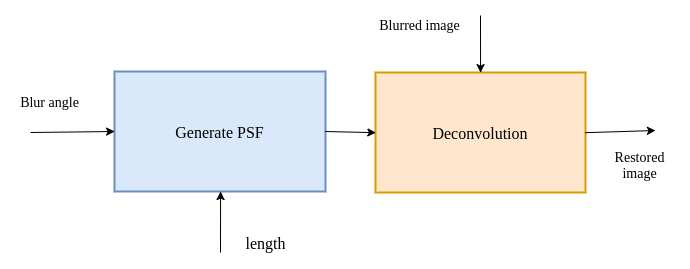
\includegraphics[width=\linewidth]{ImageRestorationMD.png}
	\caption{Image restoration}
	\label{deconv}
\end{figure}

\begin{figure}[h!]
	\centering
	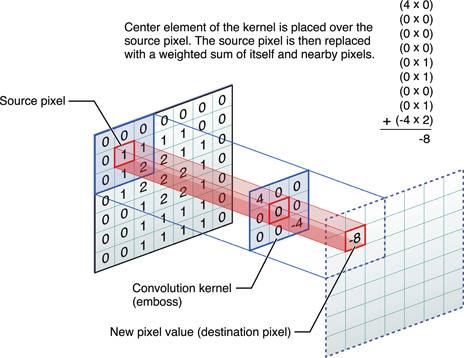
\includegraphics[width=0.75\linewidth]{kernel_convolution.jpg}
	\caption{Convolution operation that gives the output with size equal to input}
	\caption*{\small(\textit{source:https://developer.apple.com/library/content/documentation/Performance
			/Conceptual/vImage/Art/kernel\_convolution.jpg})}
	\label{fig:convolution}
\end{figure}
\subsection{GPGPU Implementation}
The motion de-blur algorithm is implemented on a system with NVIDIA GT 640 GPU and a intel i5 processor.\\
\subsubsection{Estimating blur kernel}
\begin{itemize}	
	\item Gradient of the image
	\begin{itemize}
	\item In generating PSF the first step is to find the image gradient. In this step horizontal gradient and vertical gradient of the image are calculated. From the equation \ref{gradeq}, the magnitude of horizontal and vertical gradient gives the gradient of the image.
	\item The horizontal gradient works on the next pixel and previous pixel in a row, as in Equation \ref{gradeq}. For example if a pixel in the horizontal gradient is at (x,y) then its value depends on the (x-1,y) and (x+1,y) pixels in the input image.
	\item For a pixel in horizontal gradient at boarder (0,2) then its value is decided by the (0,2) and (1,2) pixels in the input image.
	\item The vertical gradient works on the next pixel and previous pixel in the column. For example if a pixel in the vertical gradient is at (x,y) then its value depends on the (x,y-1) and (x,y+1) pixels in the input image.
	\item After the horizontal and vertical gradients are found, the magnitude can be calculated.
	\item All these three operations produce a single image gradient output. This single output can be computed by a thread at (x,y) in the grid. So output size number of threads can compute concurrently all the image gradient values.
	\item For example an image of size 640x480 the gradient output is also of same size. As shown in Figure \ref{fig:imgradient}, a block of threads with size 16x8 is proposed for computing gradient. In this case a grid with size 40x60 is created to compute all the gradient outputs.	
	\begin{figure}[h!]
		\centering
		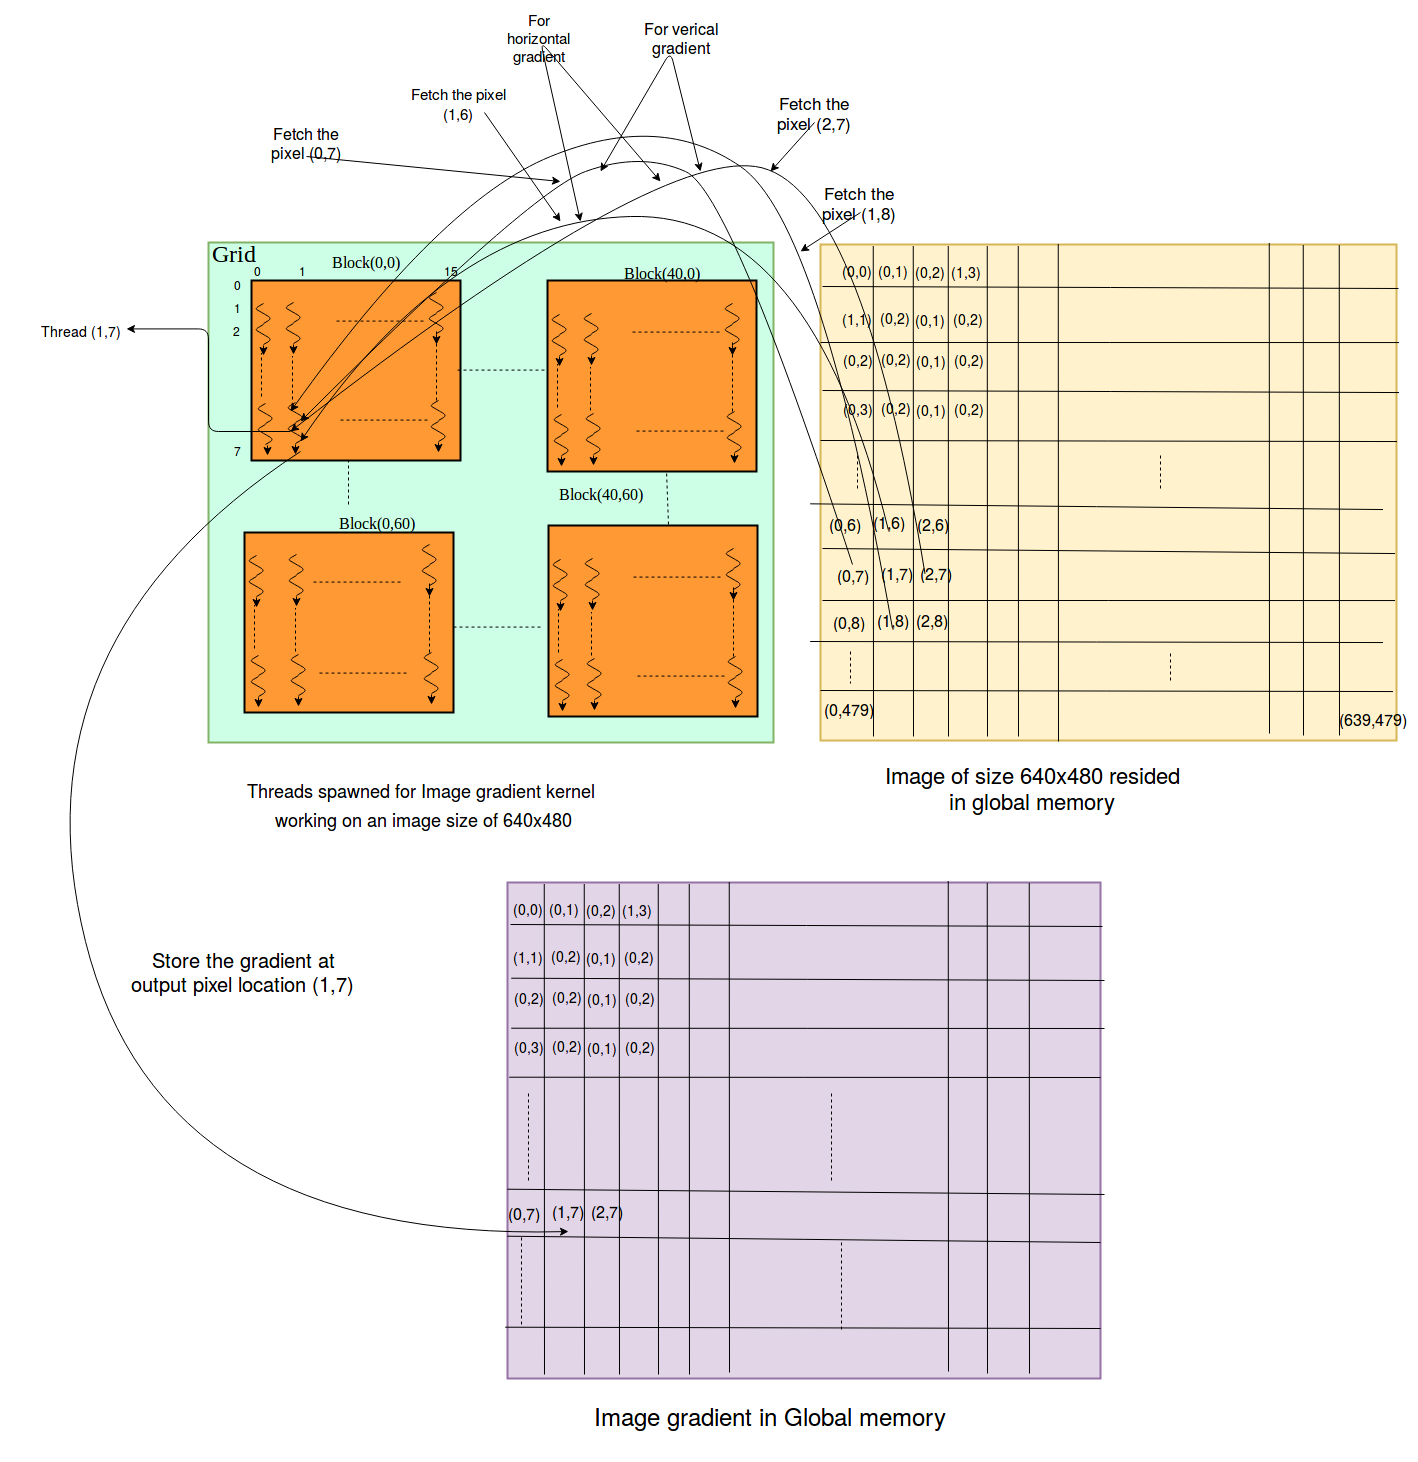
\includegraphics[width=\linewidth]{imageGradient.png}
		\caption{Thread access pattern for a kernel which finds image gradient on a image of size 640x480}
		\label{fig:imgradient}
	\end{figure}	
\end{itemize}
	\item Power spectrum of the image gradient
\begin{itemize}
	\item Power spectrum calculation in Equation \ref{pseq} is implemented using a standard CUDA library cufft.
\begin{figure}[h!]
		\centering
		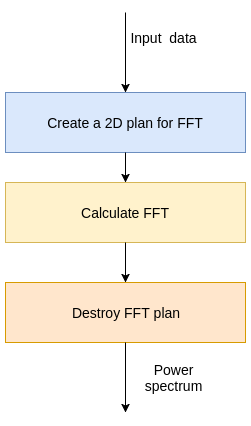
\includegraphics[width=0.4\linewidth]{powerSpectrumCalculation.png}
		\caption{CUDA cufft library usage for calculating FFT}
		\label{fig:cufft}
\end{figure}
	\item the power spectrum calculation is explained in the Figure \ref{fig:cufft}. 
\end{itemize}
\item Butterworth bandpass filtering
\begin{itemize}
	\item Butterworth bandpass filtering is applied on the power spectrum computed from the above step. It removes the unwanted frequencies from the spectrum.
	\item In this operation first a low pass filter is applied on the spectrum with a cut-off digital frequency of 3 ($d$). Then high pass filter is applied on the spectrum with cut-off digital frequency($d$) of 2. Both the filters are joined to form a band pass filter.
	\item The $n$ in the Equation \ref{bwfeq} is the order of the filter. In this case the filter is of order 5.
	\item From the Equation \ref{bwfeq}, the operating digital frequency $D(u,v)$ is calculated using the pixel location, as in Equation \ref{dist}. For a filtered output at (a,b), the operating frequency is the square of euclidean distance from the last pixel in the input image.
	\item Each output produced in the filtering is independent of the other output. An output at (a,b) can be produced with a thread at (a,b) in the grid.
	\item As shown in the Figure \ref{fig:butterworth}, for a spectrum of 640x480 the output is also of same size. A block with 16x8 threads is considered, and a grid of 40x60 is formed to compute all the outputs.
\end{itemize}
\begin{figure}[h!]
	\centering
	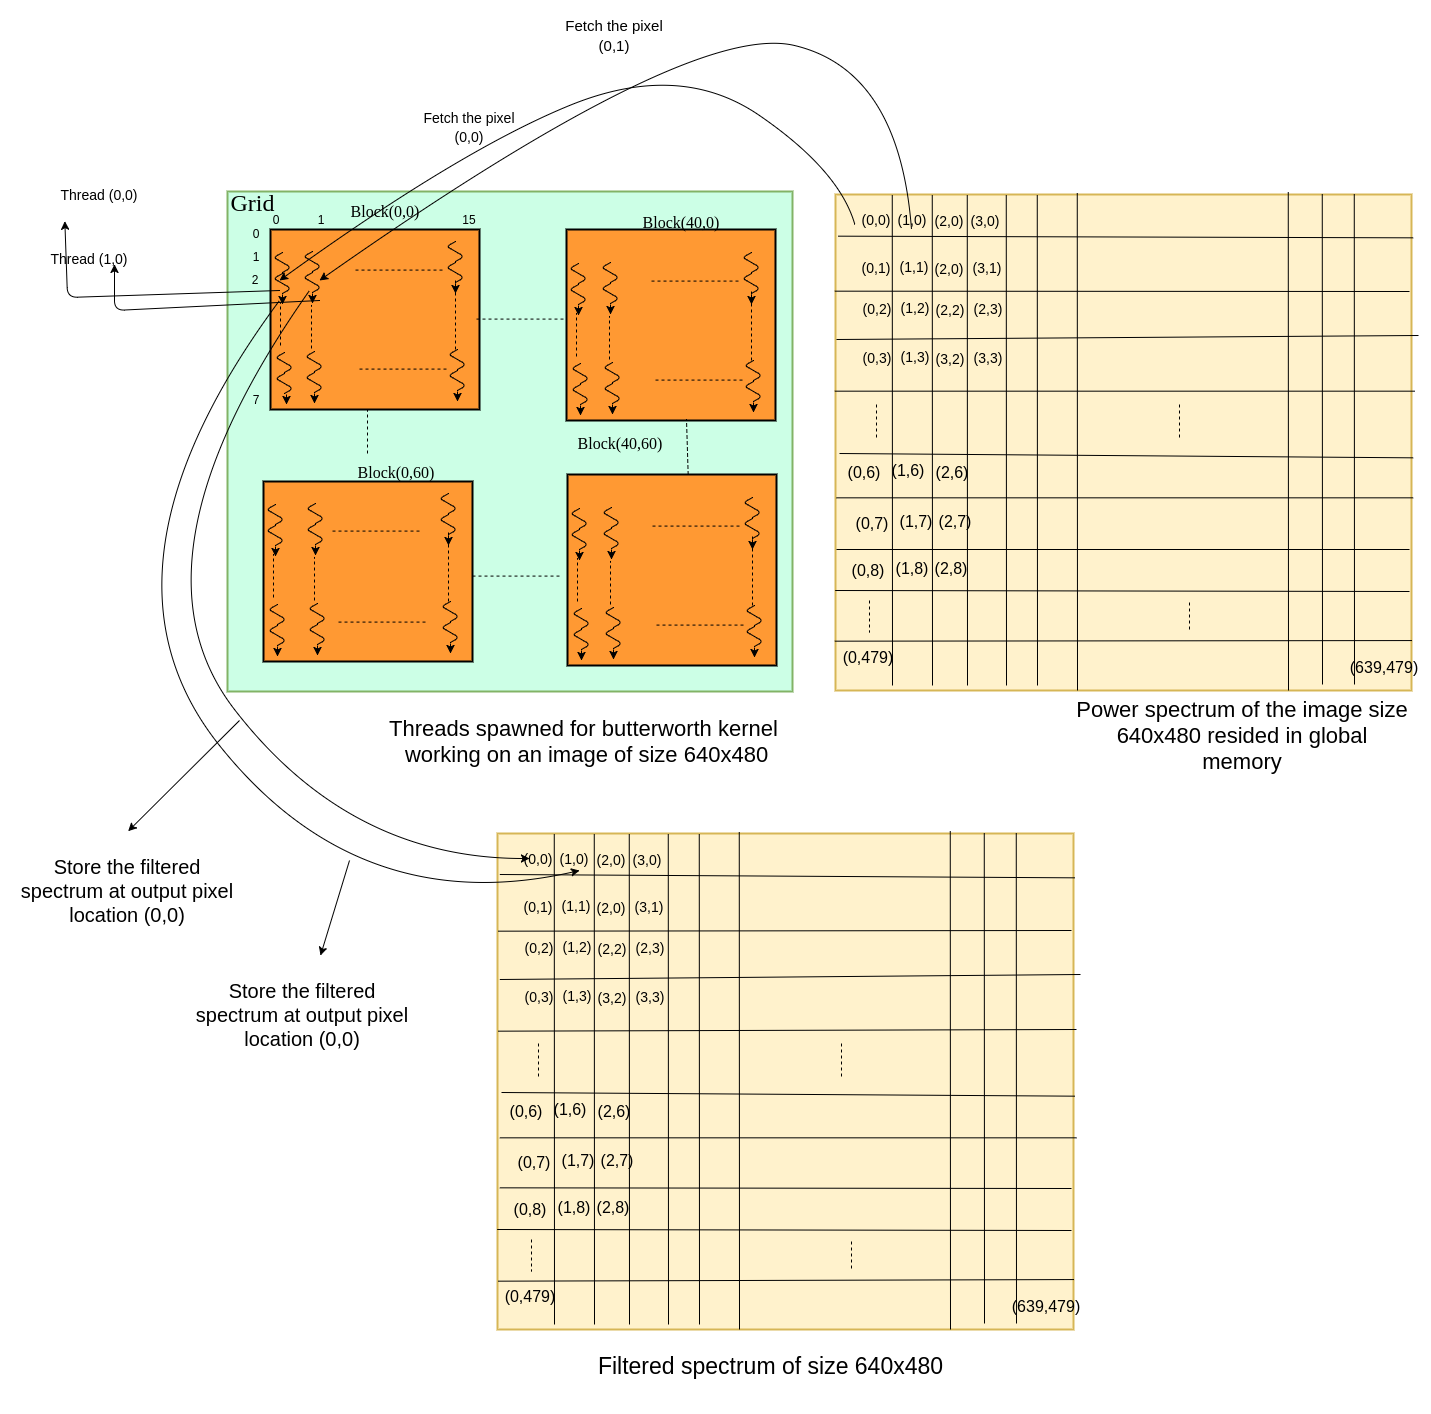
\includegraphics[width=\linewidth]{ButterworthFiltering.png}
	\caption{CUDA kernel for Butterworth band-pass filtering}
	\label{fig:butterworth}
\end{figure}
\item Radon Transform
\begin{itemize}
	\item The Radon transform works on entire image and finds the projections for each angle, as in Equation \ref{radoneq}. Radon transform will be computed for 120 angles in this algorithm starting from angle 30 to angle 150.
	\item The output size for one angle is found from the dimensions of the data. For an input of size 640x480(NxM), the output size for an angle is 1x799, calculated using Equation \ref{radszeq}. To accommodate for 121 angles output, the output size is 121x799.
	\begin{align}\label{radszeq}
	&y_c =  	\frac{(M-1)}{2}\\ &
	x_c = \frac{(N-1)}{2} \\  &
	r_h = (M-1-y_c)^2 + (N-1-x_c)^2 + 1\\&
	r = 2 \times r_h + 1
	\end{align}
	where $M$ is the height of the image, $N$ is the width of the image and $r$ is the radon transform output size for one angle.  
	\item For each pixel 4 projections are found with a 0.5 unit distance between the consecutive projections. Each projection updates output data at two locations. One at the projection and other at the 121(total number of angles) locations away from the initial projection. So a single pixel contributes at 8 locations of the radon output. These locations might intersect.
	\item For example, for a data of size 640x480, a grid of 640x480 threads can concurrently calculate projections and update the pixel data at those locations.
	\item For this case the pixel data is accumulated at the computed projections, So the accumulation operation is carried out using atomicAdd operation, this breaks some parallelism by synchronizing threads which are accessing the same location to accumulate the pixel data.
	\item A block size of 16x8 is considered, and a 2D grid of size 40x60 is created to complete the operation for all pixels.
	\item As shown in the Figure \ref{fig:radon threadaccess}, the input data size is 640x480 then the output data size is 121x799. The  thread (0,0) works on a pixel (0,0). 
	\item At an angle of $30^o$, the first projection location is (0,242), the horizontal 0.5 distant second projection is (0,242). The verical 0.5 distant third projection location is calculated as (0,243) and fourth projection with 0.5 distant in both directions is (0,243).\\
\end{itemize}
\begin{figure}[h!]
	\centering
	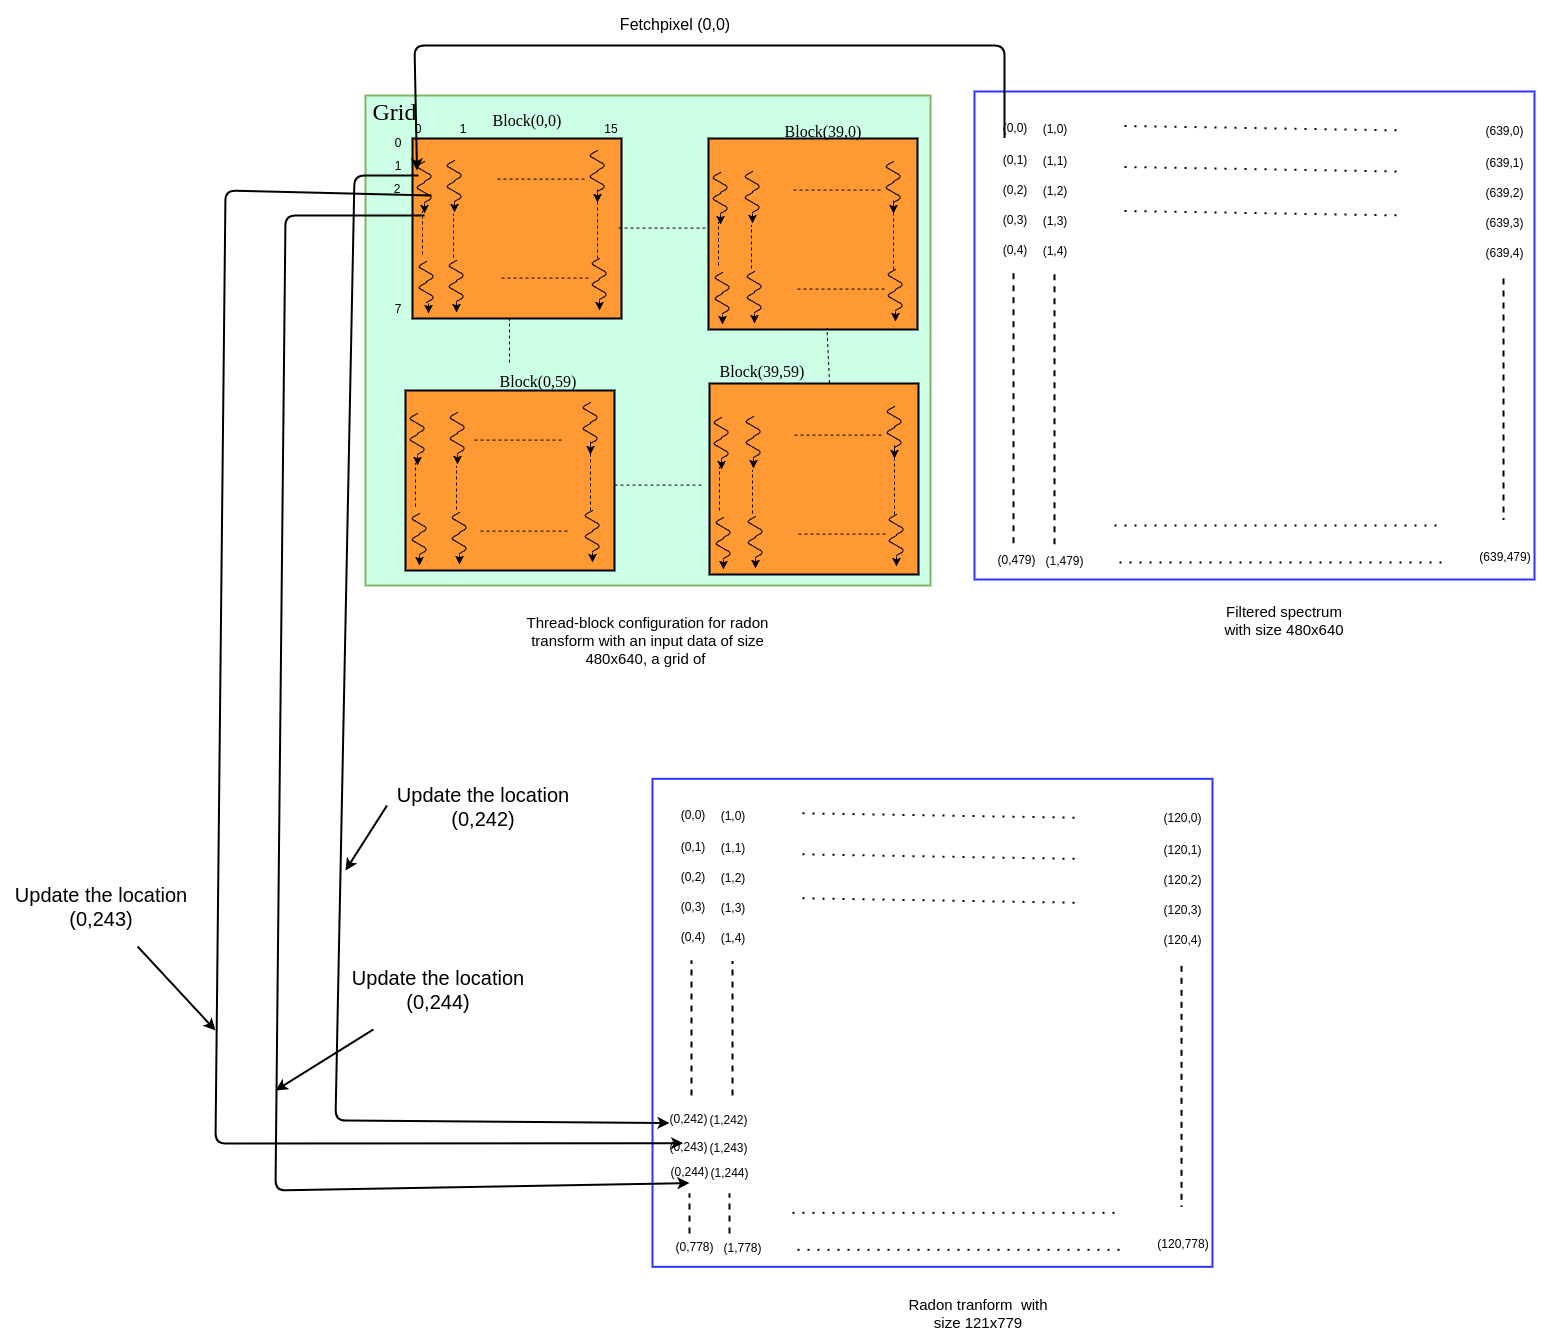
\includegraphics[width=0.75\linewidth]{radonThread.png}
	\caption{CUDA kernel for calculating Radon transform for a spectrum of size 640x480}
	\label{fig:radon threadaccess}
\end{figure}
\item Blur length calculation
\begin{itemize}
	\item The input image is first converted into frequency domain. This can be done by using standard CUDA fft library cufft , as shown in Figure \ref{fig:cufft}. 
	\item Magnitude of the power spectrum is calculated, and it is log transformed. 
	\item Finding the magnitude and log transform are pixel level operations and does not depend on the other pixels. An output at location (u,v) can be produced by a single thread at (u,v) in the grid. For a spectrum of size 640x480 the output is also of same size. A block with 16x8 threads are found to be efficient, and a grid of 40x60 is created to complete all the outputs.
	\item The result of log transform is rotated by blur angle. This data rotation is performed using OpenCV library on CPU and the blur calculation too implemented on CPU.
	\item The blur kernel estimation takes very less time on CPU and it did not qualify for data parallelism.
\end{itemize}
\end{itemize} 
\subsubsection{Deconvolution}
\begin{itemize}
	\item As explained in the algorithm, the deconvolution contains a series of convolutions.
	\item The sequence of operations are explained in the Figure .
	\begin{figure}[h!]
		\centering
		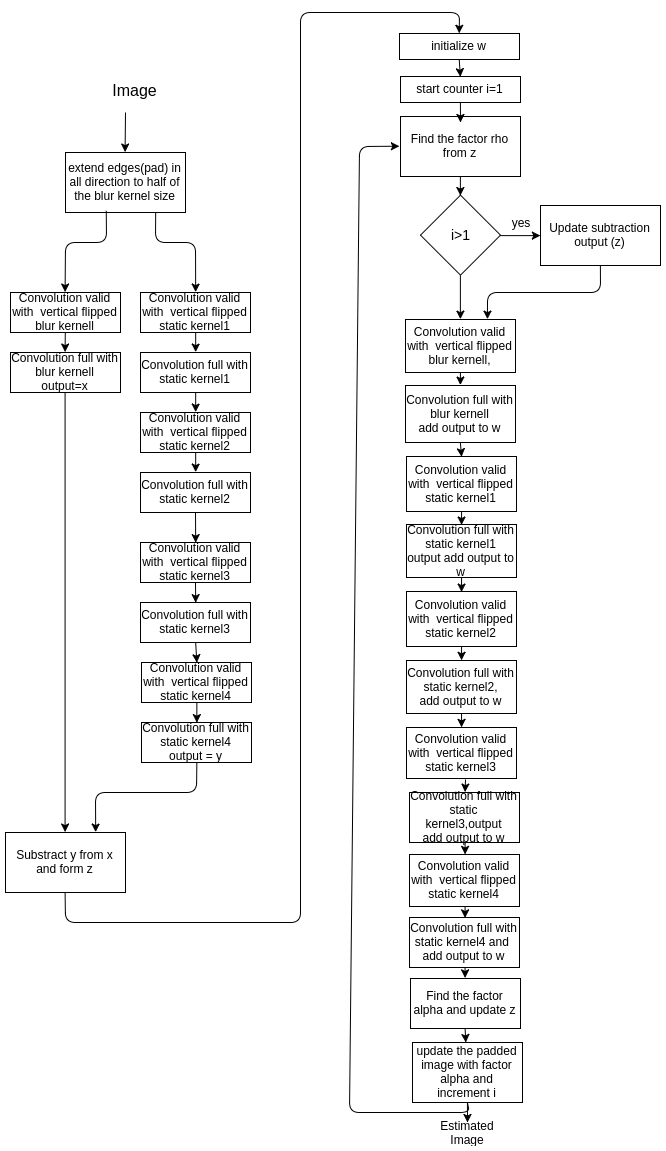
\includegraphics[width=0.8\linewidth]{deconvolutionflowchart.png}
		\caption{Sequence of operations in Deconvolution}
		\label{fig:Deconvolution flow chart}
	\end{figure}
	\item Initially the image is padded such that the boarders are extended by half kernel size. Its just a element wise copy operation. Single element copy operation can be handled by a single thread. 
	\item Creating a grid of threads with size equal to padded image then all the elements can be copied simultaneously. 16x16 threads for block considered in this case.
	\item For an image of 640x480 and a kernel with size 3x3 the output is 642x482. So a grid of 41x31 blocks is created to complete the entire operation.
	\item The padded image is subjected to valid type of convolution with the flipped blur kernel. A window of pixels from the image multiplies with the respective elements from the blur kernel. The outputs from the multiplications are accumulated to form a single convolution output.
	\item If a thread can produce an output then the output size number of threads can generate all the outputs simultaneously. But each thread will iterate over multiple times, the iteration count is controlled by the size of kernel.
	\item A block with size 16x16 is considered for convolution operation. For the above padded image with size 642x482 needs 41x31 blocks to complete the entire convolution outputs. This valid operation is shown in Figure \ref{fig:convolution kernel}.
	\item For the remaining types of convolutions, creating output size number of threads will complete the operation.
	\begin{figure}[h!]
		\centering
		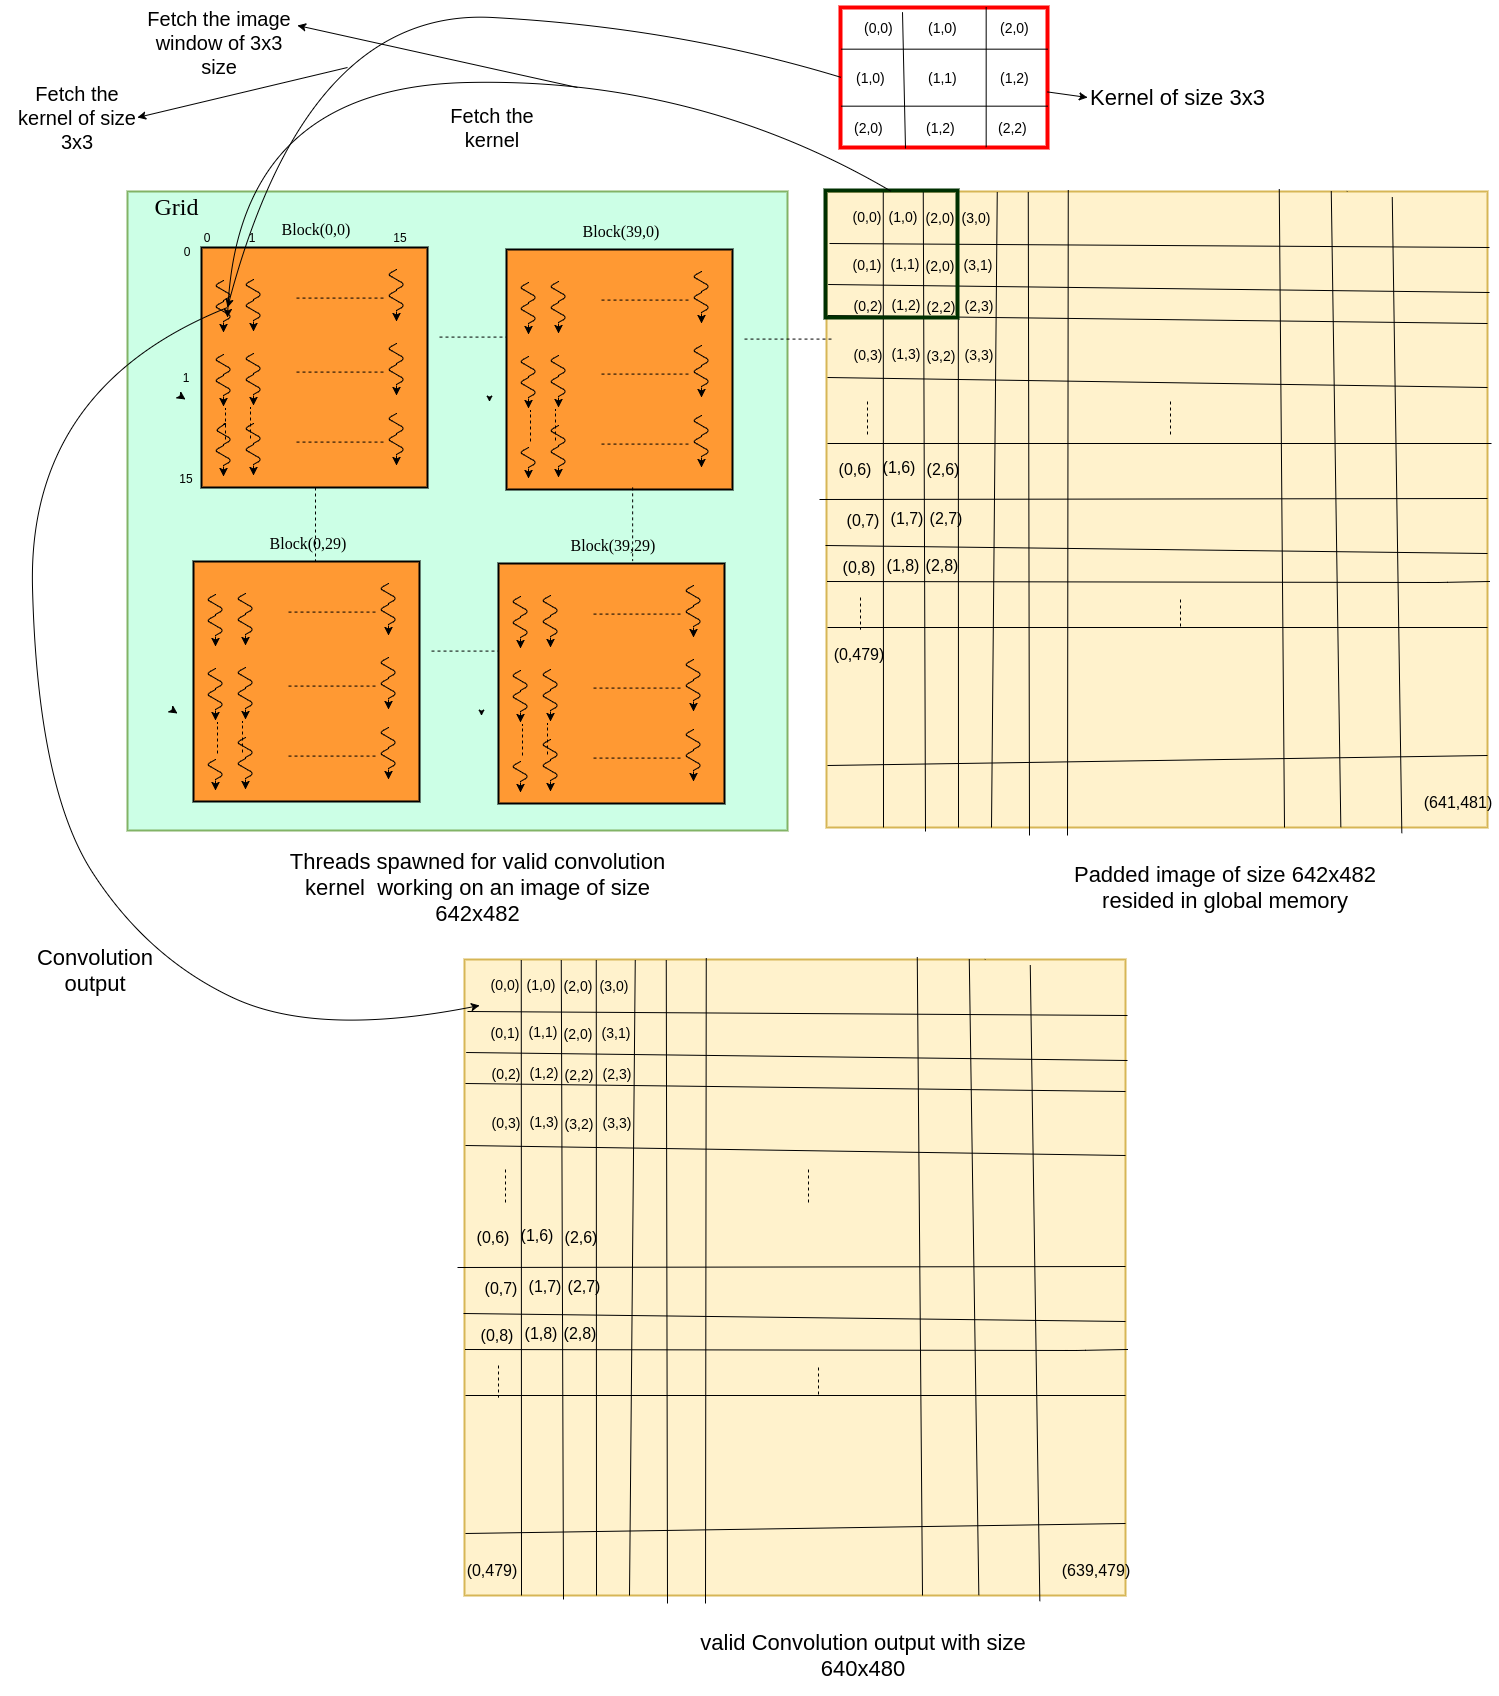
\includegraphics[width=\linewidth]{convolutionkernel.png}
		\caption{Valid type of convolution operation on GPU, thread access pattern. For an image of size 642x482 and a convolution kernel of size 3x3.}
		\label{fig:convolution kernel}
	\end{figure}
	\item For the remaining types of convolutions, creating output size number of threads will complete the convolution operations.
	\item The subtraction operation From the Figure \ref{fig:Deconvolution flow chart} is element wise. For a inputs of size 642x482, this operation can be done on GPU with a kernel with a grid of 41x31 blocks. Each block contains 16x16 threads.
	\item Calculating factor rho and alpha needs to add all the elements from the output of subtraction operation. So atomicAdd operations are used to add the elements.
\end{itemize}

\subsection{Results and Discussions}
The ported algorithm is verified against different inputs with different sizes, Table \ref{table:motion de-blur} shows the timing Performance of the motion de-blur algorithm for different sizes of input. From the Table \ref{table:motion de-blur} it is obvious to note that whenever input data is more then the speed up is more, so there is a more possibility to process this huge data in parallel.
\begin{table}[htb]
	\centering
	\resizebox{\columnwidth}{!}{%
		\begin{tabular}{|m{6em}|m{1.0cm}|m{1.0cm}|m{1.0cm}|m{1.0cm}|m{1.0cm}|m{1.0cm}|}
			\hline
			\textbf{Module}&\multicolumn{2}{c|}{\textbf{CPU(in ms)}} & \multicolumn{2}{c|}{\textbf{GPU(in ms)}} &\multicolumn{2}{c|}{\textbf{Speed Up}} \\    \cline{2-7} 
			&\textbf{480p}&\textbf{1080p}&\textbf{480p}&\textbf{1080p}&\textbf{480p}&\textbf{1080p} \\    \hline
			Gradient of the image& 	14.50 & 90.94& 0.517& 2.32& 28x & 39x\\    \hline
			Power spectrum calculation& 18.24& 154.06& 1.26& 8.81& 17x& 19x \\   \hline
			Butterworth bandpass filtering	& 22.82& 135.29& 2.39& 3.72& 10x& 36x\\   \hline
			Radon transform & 16.52& 55.12& 3.85 & 12.05 & 4.3x& 4.5x \\   \hline	
			Deconvolution \newline&320.5&3246.99&29.86&29.86&11x&17x \\   \hline
			Total timing & 1600&4200&260&580&6x&7x \\   \hline
		\end{tabular}}
		\caption{timing performance of motion de-blur algorithm}
		\label{table:motion de-blur}
	\end{table}
\begin{figure}[htb]
	{\centering
	\subfloat[input]{{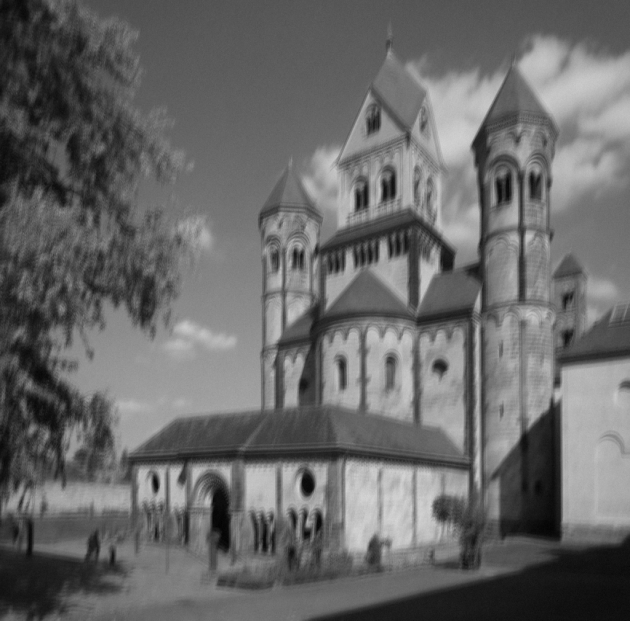
\includegraphics[width=6cm]{mdinput.png} }}%
	\qquad
	\subfloat[output]{{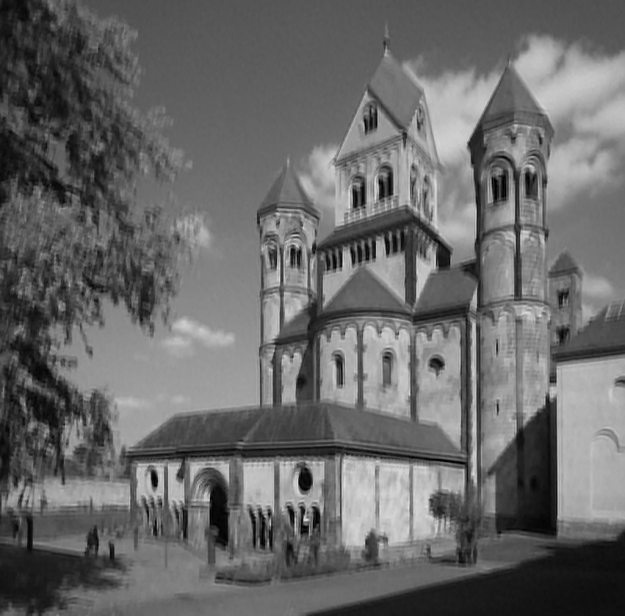
\includegraphics[width=6cm]{mdoutput.png} }}%
	\caption{Motion de-blur functional results}%
	\label{fig:motion de-blur results}%}
}
\end{figure}
\paragraph*{}From the Table \ref{table:motion de-blur} the module radon transform speed up is low. There is a dependency in the data while finding the projections, atomicAddd operation are used for this dependency, they are the main cause for less speed up. All the remaining modules data parallel so, a good speed up is observed in all the cases. All these speed up are observed without any use of texture or shared memory. Infact the there is a possibility to use shared memory in some modules, the Gradient image works on two elements and in this current scenario those two are fetched from global memory, to save one memory transaction we can use shared memory to contain data. This can be applied to convolution kernel also where a window of pixels are used for a single output.


%\end{document}
